\documentclass[twoside]{book}

% Packages required by doxygen
\usepackage{calc}
\usepackage{doxygen}
\usepackage{graphicx}
\usepackage[utf8]{inputenc}
\usepackage{makeidx}
\usepackage{multicol}
\usepackage{multirow}
\usepackage{textcomp}
\usepackage[table]{xcolor}

% Font selection
\usepackage[T1]{fontenc}
\usepackage{mathptmx}
\usepackage[scaled=.90]{helvet}
\usepackage{courier}
\usepackage{amssymb}
\usepackage{sectsty}
\renewcommand{\familydefault}{\sfdefault}
\allsectionsfont{%
  \fontseries{bc}\selectfont%
  \color{darkgray}%
}
\renewcommand{\DoxyLabelFont}{%
  \fontseries{bc}\selectfont%
  \color{darkgray}%
}

% Page & text layout
\usepackage{geometry}
\geometry{%
  a4paper,%
  top=2.5cm,%
  bottom=2.5cm,%
  left=2.5cm,%
  right=2.5cm%
}
\tolerance=750
\hfuzz=15pt
\hbadness=750
\setlength{\emergencystretch}{15pt}
\setlength{\parindent}{0cm}
\setlength{\parskip}{0.2cm}
\makeatletter
\renewcommand{\paragraph}{%
  \@startsection{paragraph}{4}{0ex}{-1.0ex}{1.0ex}{%
    \normalfont\normalsize\bfseries\SS@parafont%
  }%
}
\renewcommand{\subparagraph}{%
  \@startsection{subparagraph}{5}{0ex}{-1.0ex}{1.0ex}{%
    \normalfont\normalsize\bfseries\SS@subparafont%
  }%
}
\makeatother

% Headers & footers
\usepackage{fancyhdr}
\pagestyle{fancyplain}
\fancyhead[LE]{\fancyplain{}{\bfseries\thepage}}
\fancyhead[CE]{\fancyplain{}{}}
\fancyhead[RE]{\fancyplain{}{\bfseries\leftmark}}
\fancyhead[LO]{\fancyplain{}{\bfseries\rightmark}}
\fancyhead[CO]{\fancyplain{}{}}
\fancyhead[RO]{\fancyplain{}{\bfseries\thepage}}
\fancyfoot[LE]{\fancyplain{}{}}
\fancyfoot[CE]{\fancyplain{}{}}
\fancyfoot[RE]{\fancyplain{}{\bfseries\scriptsize Generated on Sun Mar 6 2016 21\-:21\-:15 for R\-A\-M Machine Simulator by Doxygen }}
\fancyfoot[LO]{\fancyplain{}{\bfseries\scriptsize Generated on Sun Mar 6 2016 21\-:21\-:15 for R\-A\-M Machine Simulator by Doxygen }}
\fancyfoot[CO]{\fancyplain{}{}}
\fancyfoot[RO]{\fancyplain{}{}}
\renewcommand{\footrulewidth}{0.4pt}
\renewcommand{\chaptermark}[1]{%
  \markboth{#1}{}%
}
\renewcommand{\sectionmark}[1]{%
  \markright{\thesection\ #1}%
}

% Indices & bibliography
\usepackage{natbib}
\usepackage[titles]{tocloft}
\setcounter{tocdepth}{3}
\setcounter{secnumdepth}{5}
\makeindex

% Hyperlinks (required, but should be loaded last)
\usepackage{ifpdf}
\ifpdf
  \usepackage[pdftex,pagebackref=true]{hyperref}
\else
  \usepackage[ps2pdf,pagebackref=true]{hyperref}
\fi
\hypersetup{%
  colorlinks=true,%
  linkcolor=blue,%
  citecolor=blue,%
  unicode%
}

% Custom commands
\newcommand{\clearemptydoublepage}{%
  \newpage{\pagestyle{empty}\cleardoublepage}%
}


%===== C O N T E N T S =====

\begin{document}

% Titlepage & ToC
\hypersetup{pageanchor=false}
\pagenumbering{roman}
\begin{titlepage}
\vspace*{7cm}
\begin{center}%
{\Large R\-A\-M Machine Simulator \\[1ex]\large 1 }\\
\vspace*{1cm}
{\large Generated by Doxygen 1.8.6}\\
\vspace*{0.5cm}
{\small Sun Mar 6 2016 21:21:15}\\
\end{center}
\end{titlepage}
\clearemptydoublepage
\tableofcontents
\clearemptydoublepage
\pagenumbering{arabic}
\hypersetup{pageanchor=true}

%--- Begin generated contents ---
\chapter{Hierarchical Index}
\section{Class Hierarchy}
This inheritance list is sorted roughly, but not completely, alphabetically\-:\begin{DoxyCompactList}
\item \contentsline{section}{Bubble\-Sort}{\pageref{classBubbleSort}}{}
\item \contentsline{section}{Framework}{\pageref{classFramework}}{}
\item \contentsline{section}{Problem}{\pageref{classProblem}}{}
\begin{DoxyCompactList}
\item \contentsline{section}{Fibonacci\-P}{\pageref{classFibonacciP}}{}
\item \contentsline{section}{Merge\-Sort\-P}{\pageref{classMergeSortP}}{}
\end{DoxyCompactList}
\item \contentsline{section}{Solution}{\pageref{classSolution}}{}
\begin{DoxyCompactList}
\item \contentsline{section}{Fibonacci\-S}{\pageref{classFibonacciS}}{}
\item \contentsline{section}{Merge\-Sort\-S}{\pageref{classMergeSortS}}{}
\end{DoxyCompactList}
\item \contentsline{section}{Statistics}{\pageref{classStatistics}}{}
\item \contentsline{section}{Strassen\-P}{\pageref{classStrassenP}}{}
\item \contentsline{section}{U\-I}{\pageref{classUI}}{}
\end{DoxyCompactList}

\chapter{Class Index}
\section{Class List}
Here are the classes, structs, unions and interfaces with brief descriptions\-:\begin{DoxyCompactList}
\item\contentsline{section}{\hyperlink{classBubbleSort}{Bubble\-Sort} }{\pageref{classBubbleSort}}{}
\item\contentsline{section}{\hyperlink{classFibonacciP}{Fibonacci\-P} }{\pageref{classFibonacciP}}{}
\item\contentsline{section}{\hyperlink{classFibonacciS}{Fibonacci\-S} }{\pageref{classFibonacciS}}{}
\item\contentsline{section}{\hyperlink{classFramework}{Framework} }{\pageref{classFramework}}{}
\item\contentsline{section}{\hyperlink{classMergeSortP}{Merge\-Sort\-P} }{\pageref{classMergeSortP}}{}
\item\contentsline{section}{\hyperlink{classMergeSortS}{Merge\-Sort\-S} }{\pageref{classMergeSortS}}{}
\item\contentsline{section}{\hyperlink{classProblem}{Problem} }{\pageref{classProblem}}{}
\item\contentsline{section}{\hyperlink{classSolution}{Solution} }{\pageref{classSolution}}{}
\item\contentsline{section}{\hyperlink{classStatistics}{Statistics} }{\pageref{classStatistics}}{}
\item\contentsline{section}{\hyperlink{classStrassenP}{Strassen\-P} }{\pageref{classStrassenP}}{}
\item\contentsline{section}{\hyperlink{classUI}{U\-I} }{\pageref{classUI}}{}
\end{DoxyCompactList}

\chapter{Class Documentation}
\hypertarget{classBubbleSort}{\section{Bubble\-Sort Class Reference}
\label{classBubbleSort}\index{Bubble\-Sort@{Bubble\-Sort}}
}
\subsection*{Public Member Functions}
\begin{DoxyCompactItemize}
\item 
\hypertarget{classBubbleSort_a37dbbb33b96e4f4f62548efc5ec0dc14}{{\bfseries Bubble\-Sort} (vector$<$ int $>$)}\label{classBubbleSort_a37dbbb33b96e4f4f62548efc5ec0dc14}

\item 
\hypertarget{classBubbleSort_a335ea6d7f63605717bf64bba237aa70d}{vector$<$ int $>$ {\bfseries get\-Array} ()}\label{classBubbleSort_a335ea6d7f63605717bf64bba237aa70d}

\item 
\hypertarget{classBubbleSort_a758d4700e0c0bb5c1d838ce4f7d7bb77}{void {\bfseries set\-Array\-Item} (int, int)}\label{classBubbleSort_a758d4700e0c0bb5c1d838ce4f7d7bb77}

\item 
\hypertarget{classBubbleSort_a6bad543a0fc648d1f259897e278f8edd}{void {\bfseries print} ()}\label{classBubbleSort_a6bad543a0fc648d1f259897e278f8edd}

\item 
\hypertarget{classBubbleSort_a6473a440293352ef80c837f0d8e2a045}{void {\bfseries sort} ()}\label{classBubbleSort_a6473a440293352ef80c837f0d8e2a045}

\item 
\hypertarget{classBubbleSort_a2f4e1f57a7d6132ee30b4503f1d44ae2}{int {\bfseries get\-Count} ()}\label{classBubbleSort_a2f4e1f57a7d6132ee30b4503f1d44ae2}

\end{DoxyCompactItemize}


The documentation for this class was generated from the following files\-:\begin{DoxyCompactItemize}
\item 
src/headers/Bubble\-Sort.\-hpp\item 
src/Bubble\-Sort.\-cpp\end{DoxyCompactItemize}

\hypertarget{classFibonacciP}{\section{Fibonacci\-P Class Reference}
\label{classFibonacciP}\index{Fibonacci\-P@{Fibonacci\-P}}
}
Inheritance diagram for Fibonacci\-P\-:\begin{figure}[H]
\begin{center}
\leavevmode
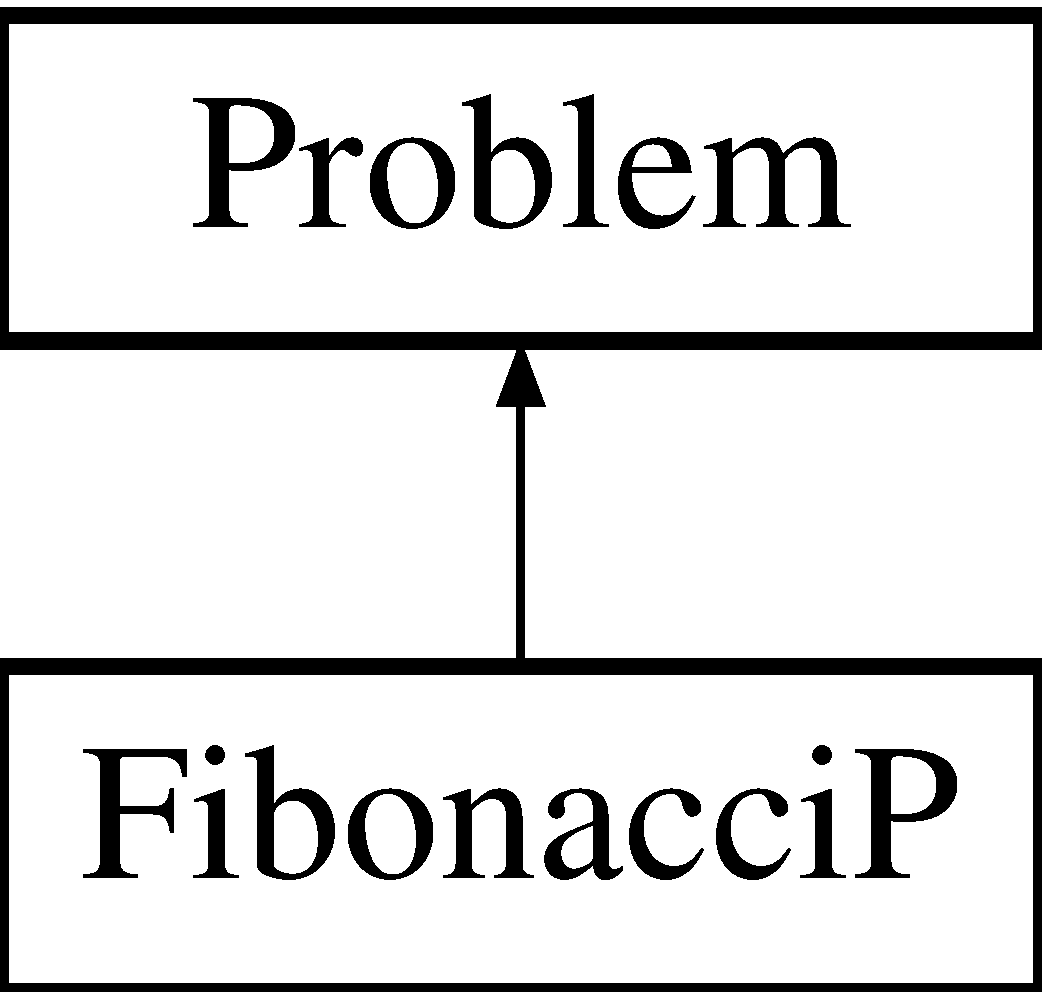
\includegraphics[height=2.000000cm]{classFibonacciP}
\end{center}
\end{figure}
\subsection*{Public Member Functions}
\begin{DoxyCompactItemize}
\item 
\hypertarget{classFibonacciP_a2ecac79d3cfb4e765b116f7d2dce04a4}{{\bfseries Fibonacci\-P} (int)}\label{classFibonacciP_a2ecac79d3cfb4e765b116f7d2dce04a4}

\item 
\hypertarget{classFibonacciP_a692b5a56f21464385b2a966dcaed4d30}{bool {\bfseries is\-Simple} ()}\label{classFibonacciP_a692b5a56f21464385b2a966dcaed4d30}

\item 
\hypertarget{classFibonacciP_afb7a04a7757d573e441928391f9c32e4}{pair$<$ \hyperlink{classProblem}{Problem} $\ast$, \hyperlink{classProblem}{Problem} $\ast$ $>$ {\bfseries decompose} ()}\label{classFibonacciP_afb7a04a7757d573e441928391f9c32e4}

\item 
\hypertarget{classFibonacciP_a71db67e416e6a43472da5e9bcc0877e0}{void {\bfseries simply\-Solve} (\hyperlink{classSolution}{Solution} $\ast$s)}\label{classFibonacciP_a71db67e416e6a43472da5e9bcc0877e0}

\end{DoxyCompactItemize}


The documentation for this class was generated from the following files\-:\begin{DoxyCompactItemize}
\item 
src/headers/Fibonacci\-P.\-hpp\item 
src/Fibonacci\-P.\-cpp\end{DoxyCompactItemize}

\hypertarget{classFibonacciS}{\section{Fibonacci\-S Class Reference}
\label{classFibonacciS}\index{Fibonacci\-S@{Fibonacci\-S}}
}
Inheritance diagram for Fibonacci\-S\-:\begin{figure}[H]
\begin{center}
\leavevmode
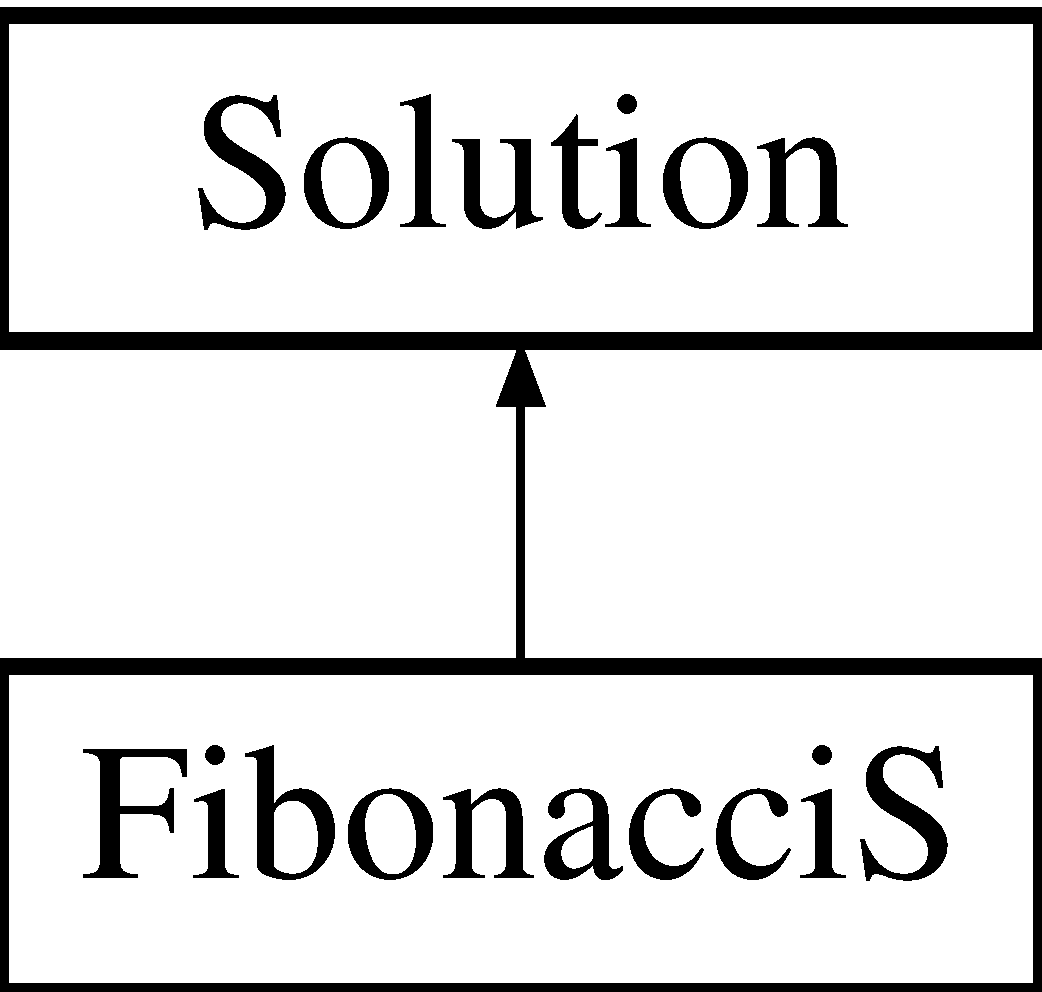
\includegraphics[height=2.000000cm]{classFibonacciS}
\end{center}
\end{figure}
\subsection*{Public Member Functions}
\begin{DoxyCompactItemize}
\item 
\hypertarget{classFibonacciS_ad4e73fb3cf507d46aab86777f2cabd9d}{void {\bfseries solve} ()}\label{classFibonacciS_ad4e73fb3cf507d46aab86777f2cabd9d}

\item 
\hypertarget{classFibonacciS_a7a3c9854b8396a160236bb15b903fecc}{void {\bfseries combine} (pair$<$ \hyperlink{classSolution}{Solution} $\ast$, \hyperlink{classSolution}{Solution} $\ast$ $>$)}\label{classFibonacciS_a7a3c9854b8396a160236bb15b903fecc}

\item 
\hypertarget{classFibonacciS_a59568b6a7ddbafa7e95f0d80979bf155}{\hyperlink{classSolution}{Solution} $\ast$ {\bfseries get\-Instance} ()}\label{classFibonacciS_a59568b6a7ddbafa7e95f0d80979bf155}

\item 
\hypertarget{classFibonacciS_a39170f654016c6f5d65e529f8441e0a4}{void {\bfseries set\-Value} (int)}\label{classFibonacciS_a39170f654016c6f5d65e529f8441e0a4}

\end{DoxyCompactItemize}


The documentation for this class was generated from the following files\-:\begin{DoxyCompactItemize}
\item 
src/headers/Fibonacci\-S.\-hpp\item 
src/Fibonacci\-S.\-cpp\end{DoxyCompactItemize}

\hypertarget{classFramework}{\section{Framework Class Reference}
\label{classFramework}\index{Framework@{Framework}}
}
\subsection*{Public Member Functions}
\begin{DoxyCompactItemize}
\item 
\hypertarget{classFramework_aaed170a2954c53ce3fc2818ada396ad4}{void {\bfseries divide\-And\-Conquer} (\hyperlink{classProblem}{Problem} $\ast$p, \hyperlink{classSolution}{Solution} $\ast$s)}\label{classFramework_aaed170a2954c53ce3fc2818ada396ad4}

\end{DoxyCompactItemize}


The documentation for this class was generated from the following files\-:\begin{DoxyCompactItemize}
\item 
src/headers/Framework.\-hpp\item 
src/Framework.\-cpp\end{DoxyCompactItemize}

\hypertarget{classMergeSortP}{\section{Merge\-Sort\-P Class Reference}
\label{classMergeSortP}\index{Merge\-Sort\-P@{Merge\-Sort\-P}}
}
Inheritance diagram for Merge\-Sort\-P\-:\begin{figure}[H]
\begin{center}
\leavevmode
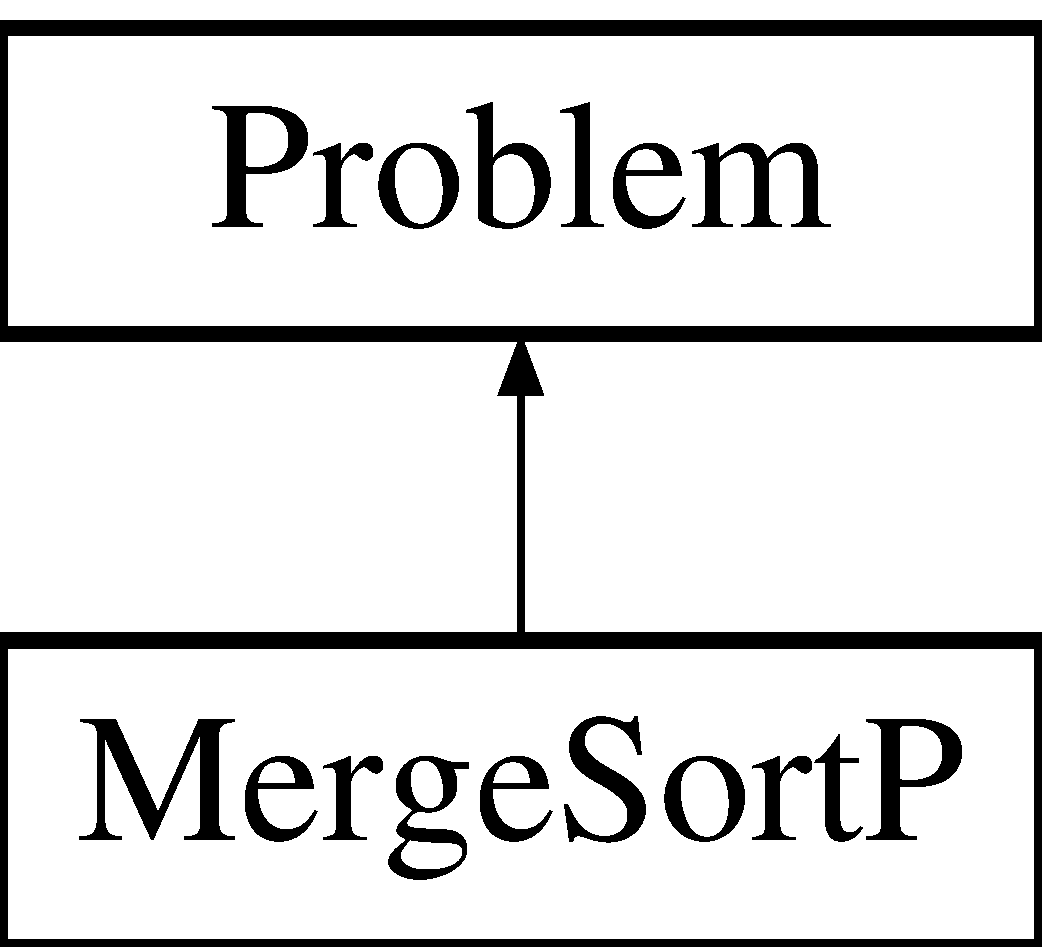
\includegraphics[height=2.000000cm]{classMergeSortP}
\end{center}
\end{figure}
\subsection*{Public Member Functions}
\begin{DoxyCompactItemize}
\item 
\hypertarget{classMergeSortP_ab7c5a3031e2b78cea226a29f9b7d6d5b}{{\bfseries Merge\-Sort\-P} (vector$<$ int $>$)}\label{classMergeSortP_ab7c5a3031e2b78cea226a29f9b7d6d5b}

\item 
\hypertarget{classMergeSortP_a7a212b9f90c98f951b71f6e56b9f653c}{bool {\bfseries is\-Simple} ()}\label{classMergeSortP_a7a212b9f90c98f951b71f6e56b9f653c}

\item 
\hypertarget{classMergeSortP_a362a085252146bb26efab7403d4a8478}{pair$<$ \hyperlink{classProblem}{Problem} $\ast$, \hyperlink{classProblem}{Problem} $\ast$ $>$ {\bfseries decompose} ()}\label{classMergeSortP_a362a085252146bb26efab7403d4a8478}

\item 
\hypertarget{classMergeSortP_ad107af3328d6ec7194d840bf73416ef7}{void {\bfseries simply\-Solve} (\hyperlink{classSolution}{Solution} $\ast$s)}\label{classMergeSortP_ad107af3328d6ec7194d840bf73416ef7}

\item 
\hypertarget{classMergeSortP_a9c953d6bbf847cdd1651a4cce4fb9423}{int \& {\bfseries get\-Count} ()}\label{classMergeSortP_a9c953d6bbf847cdd1651a4cce4fb9423}

\item 
\hypertarget{classMergeSortP_ada4b59301540fadc232bff2b20bf7bf5}{void {\bfseries reset\-Count} ()}\label{classMergeSortP_ada4b59301540fadc232bff2b20bf7bf5}

\end{DoxyCompactItemize}


The documentation for this class was generated from the following files\-:\begin{DoxyCompactItemize}
\item 
src/headers/Merge\-Sort\-P.\-hpp\item 
src/Merge\-Sort\-P.\-cpp\end{DoxyCompactItemize}

\hypertarget{classMergeSortS}{\section{Merge\-Sort\-S Class Reference}
\label{classMergeSortS}\index{Merge\-Sort\-S@{Merge\-Sort\-S}}
}
Inheritance diagram for Merge\-Sort\-S\-:\begin{figure}[H]
\begin{center}
\leavevmode
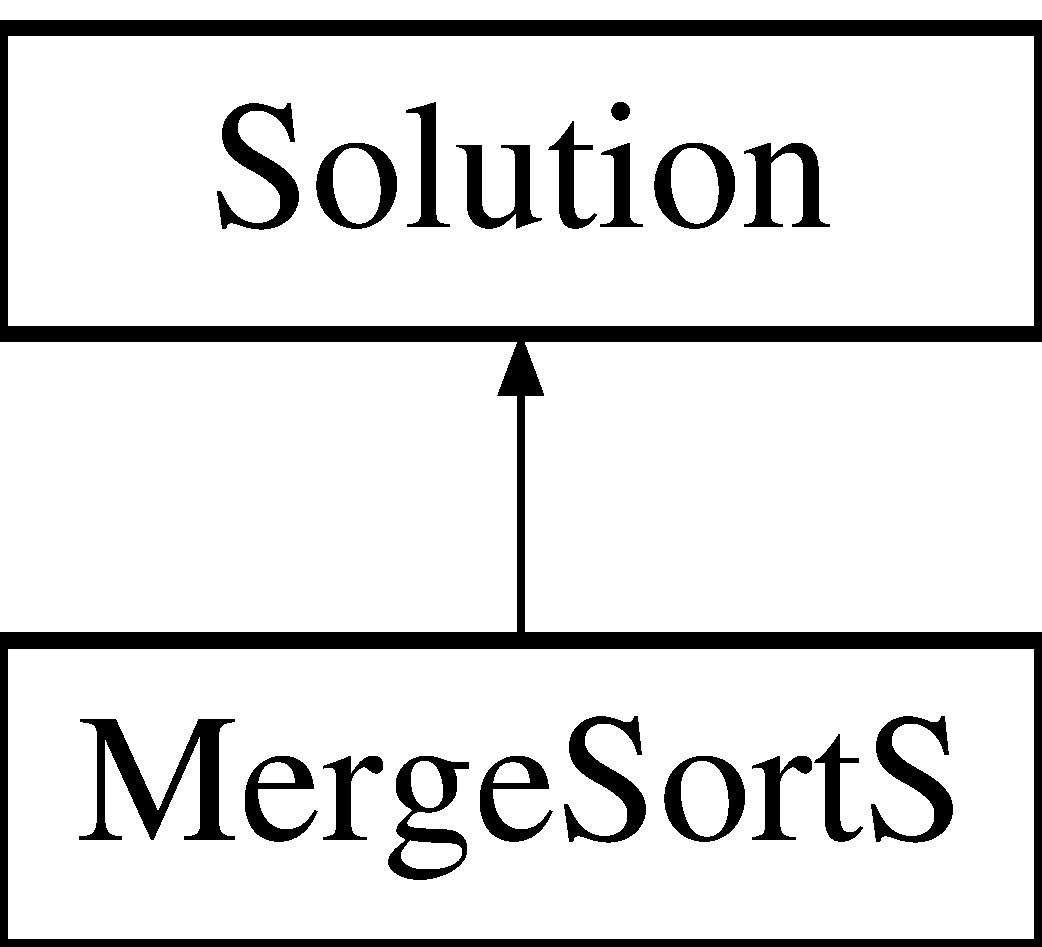
\includegraphics[height=2.000000cm]{classMergeSortS}
\end{center}
\end{figure}
\subsection*{Public Member Functions}
\begin{DoxyCompactItemize}
\item 
\hypertarget{classMergeSortS_a0609d7b00651a4fdd4aa60678e2c07d5}{void {\bfseries solve} ()}\label{classMergeSortS_a0609d7b00651a4fdd4aa60678e2c07d5}

\item 
\hypertarget{classMergeSortS_aad9bbe320dac4eedfa3fa0a435670b50}{void {\bfseries combine} (pair$<$ \hyperlink{classSolution}{Solution} $\ast$, \hyperlink{classSolution}{Solution} $\ast$ $>$)}\label{classMergeSortS_aad9bbe320dac4eedfa3fa0a435670b50}

\item 
\hypertarget{classMergeSortS_a6e8f5575eb38fe2eb3e57138b4fd47f5}{\hyperlink{classSolution}{Solution} $\ast$ {\bfseries get\-Instance} ()}\label{classMergeSortS_a6e8f5575eb38fe2eb3e57138b4fd47f5}

\item 
\hypertarget{classMergeSortS_a25499fb864f86ad8953a7dbef4fcf76e}{void {\bfseries set\-Value} (vector$<$ int $>$)}\label{classMergeSortS_a25499fb864f86ad8953a7dbef4fcf76e}

\end{DoxyCompactItemize}


The documentation for this class was generated from the following files\-:\begin{DoxyCompactItemize}
\item 
src/headers/Merge\-Sort\-S.\-hpp\item 
src/Merge\-Sort\-S.\-cpp\end{DoxyCompactItemize}

\hypertarget{classProblem}{\section{Problem Class Reference}
\label{classProblem}\index{Problem@{Problem}}
}
Inheritance diagram for Problem\-:\begin{figure}[H]
\begin{center}
\leavevmode
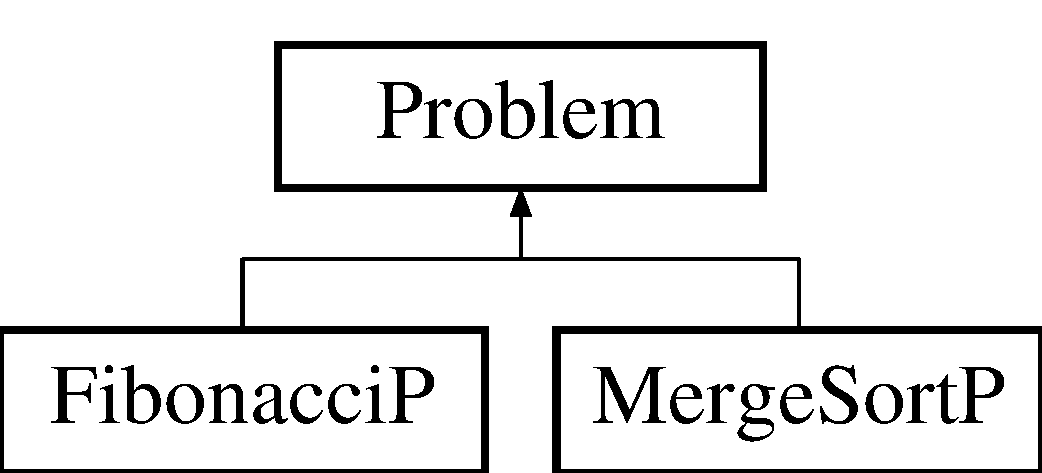
\includegraphics[height=2.000000cm]{classProblem}
\end{center}
\end{figure}
\subsection*{Public Member Functions}
\begin{DoxyCompactItemize}
\item 
\hypertarget{classProblem_abac3f602fb70288f129c6cbd8286c7b8}{virtual bool {\bfseries is\-Simple} ()}\label{classProblem_abac3f602fb70288f129c6cbd8286c7b8}

\item 
\hypertarget{classProblem_a92f3e992bcaef1abc58841515a758099}{virtual pair$<$ \hyperlink{classProblem}{Problem} \\*
$\ast$, \hyperlink{classProblem}{Problem} $\ast$ $>$ {\bfseries decompose} ()}\label{classProblem_a92f3e992bcaef1abc58841515a758099}

\item 
\hypertarget{classProblem_a342fcc85680fbc4f1a0396c25377ad81}{virtual void {\bfseries simply\-Solve} (\hyperlink{classSolution}{Solution} $\ast$s)}\label{classProblem_a342fcc85680fbc4f1a0396c25377ad81}

\item 
\hypertarget{classProblem_a64a4bd847dc5fcc78693898338bd9d8d}{virtual int \& {\bfseries get\-Count} ()}\label{classProblem_a64a4bd847dc5fcc78693898338bd9d8d}

\item 
\hypertarget{classProblem_a75980148545f29b70a746ad86fab590d}{virtual void {\bfseries reset\-Count} ()}\label{classProblem_a75980148545f29b70a746ad86fab590d}

\end{DoxyCompactItemize}


The documentation for this class was generated from the following files\-:\begin{DoxyCompactItemize}
\item 
src/headers/Problem.\-hpp\item 
src/Problem.\-cpp\end{DoxyCompactItemize}

\hypertarget{classSolution}{\section{Solution Class Reference}
\label{classSolution}\index{Solution@{Solution}}
}
Inheritance diagram for Solution\-:\begin{figure}[H]
\begin{center}
\leavevmode
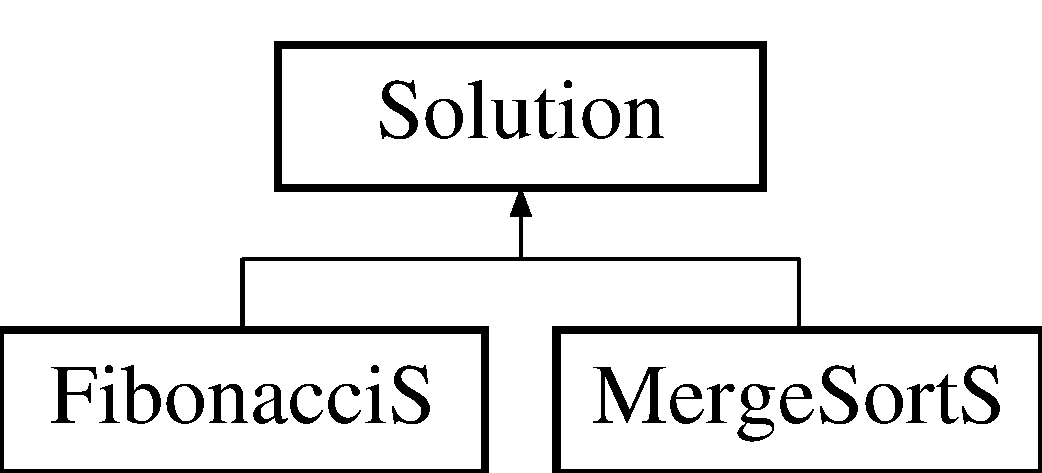
\includegraphics[height=2.000000cm]{classSolution}
\end{center}
\end{figure}
\subsection*{Public Member Functions}
\begin{DoxyCompactItemize}
\item 
\hypertarget{classSolution_ab69c19a449ed2f7289c8c0b4d8690d1d}{virtual void {\bfseries solve} ()}\label{classSolution_ab69c19a449ed2f7289c8c0b4d8690d1d}

\item 
\hypertarget{classSolution_add7d3c93aa7c6dd9e7e2def61d706ec9}{virtual void {\bfseries combine} (pair$<$ \hyperlink{classSolution}{Solution} $\ast$, \hyperlink{classSolution}{Solution} $\ast$ $>$)}\label{classSolution_add7d3c93aa7c6dd9e7e2def61d706ec9}

\item 
\hypertarget{classSolution_a654dea68c595ae8065a6b563865c23c6}{virtual \hyperlink{classSolution}{Solution} $\ast$ {\bfseries get\-Instance} ()}\label{classSolution_a654dea68c595ae8065a6b563865c23c6}

\end{DoxyCompactItemize}


The documentation for this class was generated from the following files\-:\begin{DoxyCompactItemize}
\item 
src/headers/Solution.\-hpp\item 
src/Solution.\-cpp\end{DoxyCompactItemize}

\hypertarget{classStatistics}{\section{Statistics Class Reference}
\label{classStatistics}\index{Statistics@{Statistics}}
}
\subsection*{Public Member Functions}
\begin{DoxyCompactItemize}
\item 
\hypertarget{classStatistics_aca73ba8ebcbdc237d2829a2fb377e21b}{int {\bfseries get\-First} ()}\label{classStatistics_aca73ba8ebcbdc237d2829a2fb377e21b}

\item 
\hypertarget{classStatistics_a5f8fe56aa20a6f420d26ab4f87629a03}{int {\bfseries get\-Second} ()}\label{classStatistics_a5f8fe56aa20a6f420d26ab4f87629a03}

\item 
\hypertarget{classStatistics_ac22edc61027bc702dbddc0287127de54}{int {\bfseries get\-Testing\-Cases\-Number} ()}\label{classStatistics_ac22edc61027bc702dbddc0287127de54}

\item 
\hypertarget{classStatistics_ace2a57535ff9c70d4b8f187c49f7290b}{void {\bfseries set\-Testing\-Cases\-Number} (int num)}\label{classStatistics_ace2a57535ff9c70d4b8f187c49f7290b}

\item 
\hypertarget{classStatistics_a0487edd5c45d29847a7f83ba43974ee7}{void {\bfseries add\-To\-First} (int num)}\label{classStatistics_a0487edd5c45d29847a7f83ba43974ee7}

\item 
\hypertarget{classStatistics_a74e32bb790dd6340d9213cc500878b44}{void {\bfseries add\-To\-Second} (int num)}\label{classStatistics_a74e32bb790dd6340d9213cc500878b44}

\item 
\hypertarget{classStatistics_a4faa80fa024777d57b6fa4b3559eec0a}{void {\bfseries clear} ()}\label{classStatistics_a4faa80fa024777d57b6fa4b3559eec0a}

\end{DoxyCompactItemize}


The documentation for this class was generated from the following files\-:\begin{DoxyCompactItemize}
\item 
src/headers/Statistics.\-hpp\item 
src/Statistics.\-cpp\end{DoxyCompactItemize}

\hypertarget{classStrassenP}{\section{Strassen\-P Class Reference}
\label{classStrassenP}\index{Strassen\-P@{Strassen\-P}}
}
\subsection*{Public Member Functions}
\begin{DoxyCompactItemize}
\item 
\hypertarget{classStrassenP_af667546e759d6dbe9450123456d837f9}{{\bfseries Strassen\-P} (vector$<$ vector$<$ int $>$ $>$, vector$<$ vector$<$ int $>$ $>$)}\label{classStrassenP_af667546e759d6dbe9450123456d837f9}

\item 
\hypertarget{classStrassenP_a90a8518a66195a450fa092f81b2afc53}{vector$<$ vector$<$ int $>$ $>$ {\bfseries get\-Matrix\-A} ()}\label{classStrassenP_a90a8518a66195a450fa092f81b2afc53}

\item 
\hypertarget{classStrassenP_ab3f3e1e534100d093f694a15d46da9e1}{vector$<$ vector$<$ int $>$ $>$ {\bfseries get\-Matrix\-B} ()}\label{classStrassenP_ab3f3e1e534100d093f694a15d46da9e1}

\item 
\hypertarget{classStrassenP_aeefdfffdfcd6b50b53ccb5219c73f8bc}{vector$<$ vector$<$ int $>$ $>$ {\bfseries get\-Matrix\-C} ()}\label{classStrassenP_aeefdfffdfcd6b50b53ccb5219c73f8bc}

\item 
\hypertarget{classStrassenP_ad2febb1be9ba3f9713d60c6af1c1ca8a}{void {\bfseries set\-Matrix\-C} (vector$<$ vector$<$ int $>$ $>$ new\-C)}\label{classStrassenP_ad2febb1be9ba3f9713d60c6af1c1ca8a}

\item 
\hypertarget{classStrassenP_a49d9cae3084d28dc7a50dea925235b63}{int {\bfseries get\-Size} ()}\label{classStrassenP_a49d9cae3084d28dc7a50dea925235b63}

\item 
\hypertarget{classStrassenP_ac47e1183af813fac2160281bcb7308dd}{bool {\bfseries is\-Simple} (int)}\label{classStrassenP_ac47e1183af813fac2160281bcb7308dd}

\item 
\hypertarget{classStrassenP_af3fe4a89fe5b4743c99965881afc6f62}{void {\bfseries simply\-Solve} (vector$<$ vector$<$ int $>$ $>$, vector$<$ vector$<$ int $>$ $>$, vector$<$ vector$<$ int $>$ $>$ \&, int)}\label{classStrassenP_af3fe4a89fe5b4743c99965881afc6f62}

\item 
\hypertarget{classStrassenP_aecdf8438ab2f8d1cf16e184f3b0911a2}{void {\bfseries init} ()}\label{classStrassenP_aecdf8438ab2f8d1cf16e184f3b0911a2}

\item 
\hypertarget{classStrassenP_afaadbd17121fbaa8884e951a10c82fba}{void {\bfseries solve\-Recursively} (vector$<$ vector$<$ int $>$ $>$ \&, vector$<$ vector$<$ int $>$ $>$ \&, vector$<$ vector$<$ int $>$ $>$ \&, int)}\label{classStrassenP_afaadbd17121fbaa8884e951a10c82fba}

\item 
\hypertarget{classStrassenP_aa1f4f752c28183d6310fb0a18d20533a}{void {\bfseries solve} (vector$<$ vector$<$ int $>$ $>$ \&, vector$<$ vector$<$ int $>$ $>$ \&, vector$<$ vector$<$ int $>$ $>$ \&, int)}\label{classStrassenP_aa1f4f752c28183d6310fb0a18d20533a}

\item 
\hypertarget{classStrassenP_af9f8ad257710837a26afe3879ce36814}{void {\bfseries print} ()}\label{classStrassenP_af9f8ad257710837a26afe3879ce36814}

\item 
\hypertarget{classStrassenP_a61384cf91d4efda64cb12e032202a85d}{void {\bfseries sub} (vector$<$ vector$<$ int $>$ $>$, vector$<$ vector$<$ int $>$ $>$, vector$<$ vector$<$ int $>$ $>$ \&, int)}\label{classStrassenP_a61384cf91d4efda64cb12e032202a85d}

\item 
\hypertarget{classStrassenP_a71e5b5e85678d1c95c6c69861697e32c}{void {\bfseries sum} (vector$<$ vector$<$ int $>$ $>$, vector$<$ vector$<$ int $>$ $>$, vector$<$ vector$<$ int $>$ $>$ \&, int)}\label{classStrassenP_a71e5b5e85678d1c95c6c69861697e32c}

\item 
\hypertarget{classStrassenP_a36890bb07ef6299dc85e7f9cab54aab7}{void {\bfseries basic\-Mul} (vector$<$ vector$<$ int $>$ $>$, vector$<$ vector$<$ int $>$ $>$, vector$<$ vector$<$ int $>$ $>$ \&, int)}\label{classStrassenP_a36890bb07ef6299dc85e7f9cab54aab7}

\end{DoxyCompactItemize}


The documentation for this class was generated from the following files\-:\begin{DoxyCompactItemize}
\item 
src/headers/Strassen\-P.\-hpp\item 
src/Strassen\-P.\-cpp\end{DoxyCompactItemize}

\hypertarget{classUI}{\section{U\-I Class Reference}
\label{classUI}\index{U\-I@{U\-I}}
}
\subsection*{Public Member Functions}
\begin{DoxyCompactItemize}
\item 
\hypertarget{classUI_a2277decc2cba013de2fbb5a64fbc1543}{void {\bfseries init} ()}\label{classUI_a2277decc2cba013de2fbb5a64fbc1543}

\item 
\hypertarget{classUI_ae84bafbd5341a1e6759a89c7ccad0ae8}{void {\bfseries show\-Menu} ()}\label{classUI_ae84bafbd5341a1e6759a89c7ccad0ae8}

\item 
\hypertarget{classUI_ad929a7c850dcd2ff808f2c59be212f6a}{void {\bfseries wait\-For\-Key} ()}\label{classUI_ad929a7c850dcd2ff808f2c59be212f6a}

\item 
\hypertarget{classUI_ae27c365b6cd8088b7f33a4ac1e6fae3b}{void {\bfseries generate\-Random\-Vectors} (int problem\-Size)}\label{classUI_ae27c365b6cd8088b7f33a4ac1e6fae3b}

\item 
\hypertarget{classUI_ae904f4472bdce87941827fff6c90c1e1}{void {\bfseries show\-Table} ()}\label{classUI_ae904f4472bdce87941827fff6c90c1e1}

\item 
\hypertarget{classUI_a2c28ee34efdf4c0e6e93cbc7e0314cbc}{void {\bfseries do\-Full\-Study} ()}\label{classUI_a2c28ee34efdf4c0e6e93cbc7e0314cbc}

\end{DoxyCompactItemize}


The documentation for this class was generated from the following files\-:\begin{DoxyCompactItemize}
\item 
src/headers/U\-I.\-hpp\item 
src/U\-I.\-cpp\end{DoxyCompactItemize}

%--- End generated contents ---

% Index
\newpage
\phantomsection
\addcontentsline{toc}{chapter}{Index}
\printindex

\end{document}
